\documentclass[handout]{beamer}
\usepackage{amsmath,amssymb,amsthm,array}
\usepackage{bm}
\usepackage{multirow}
\usepackage{multicol}
\usepackage{changepage}
\usepackage{algorithm}
\usepackage{hyperref}
\usepackage{algorithmic}
\usepackage[normalem]{ulem}
\usepackage{fontspec}
\usepackage{numprint}

\setmainfont{CMU Serif}
\setsansfont{CMU Sans Serif}
\newfontfamily{\greekfont}{CMU Serif}
\newfontfamily{\greekfontsf}{CMU Sans Serif}

\usetheme{Rochester}
\usecolortheme{crane}

\setbeamertemplate{navigation symbols}{}
\title{Κρυπτο Ψηφοφορίες}
\author{Παναγιώτης Γροντάς}
\date{}
\defbeamertemplate*{footline}{shadow theme}
{%
  \leavevmode%
  \hbox{\begin{beamercolorbox}[wd=.5\paperwidth,ht=2.5ex,dp=1.125ex,leftskip=.3cm plus1fil,rightskip=.3cm]{author in head/foot}%
    \usebeamerfont{author in head/foot}\insertframenumber\,/\,\inserttotalframenumber\hfill  (\insertshortinstitute)
  \end{beamercolorbox}%
  \begin{beamercolorbox}[wd=.5\paperwidth,ht=2.5ex,dp=1.125ex,leftskip=.3cm,rightskip=.3cm plus1fil]{title in head/foot}%
    \usebeamerfont{title in head/foot}\insertshorttitle%
  \end{beamercolorbox}}%
  \vskip0pt%
}
\institute{ΕΜΠ - Κρυπτογραφία - (2016-2017)}

 \hypersetup{
  pdfauthor={Panagiotis Grontas},
  pdftitle={Electronic Voting},
  colorlinks=true,
  urlcolor=blue,
  linkcolor=white
}

\setlength{\columnseprule}{0.4pt}
\begin{document}
\newcommand{\xor}{ \oplus }
\newcommand{\MSG}{ \mathtt{M} }
\newcommand{\KEY}{ \mathtt{K} }
\newcommand{\CPH}{ \mathtt{C} }
\newcommand{\keygen}{\mathtt{KeyGen}}
\newcommand{\enc}{\mathtt{Encrypt}}
\newcommand{\dec}{\mathtt{Decrypt}}
\newcommand{\adv}{$\mathcal{A} \,$ }
\newcommand{\advb}{$\mathcal{B} \,$ }
\newcommand{\chal}{$\mathcal{C} \,$ }
\newcommand{\cs}{$\mathcal{CS} \,$ }
\newcommand{\zns}{  \mathbb{Z}^*_n }
\newcommand{\zs}[1]{  \mathbb{Z}^*_{#1} }

\newcommand{\green}[1]{\textcolor{teal}{#1}}
\newcommand{\Green}[1]{\textcolor{Teal}{#1}}
\newcommand{\ForestGreen}[1]{\textcolor{ForestGreen}{#1}}
\newcommand{\blue}[1]{\textcolor{blue}{#1}}
\newcommand{\magenta}[1]{\textcolor{magenta}{#1}}
\newcommand{\cyan}[1]{\textcolor{cyan}{#1}}

\newcommand{\twopartdef}[4]
{ 
		\begin{cases}
			#1 , #2 \\
			#3 , #4
		\end{cases} 
}
\begin{frame}
\titlepage
\end{frame}


\npthousandsep{ }

\begin{section}{Εισαγωγή}

\begin{frame}{Είπαν για τις (ηλεκτρονικές) ψηφοφορίες...}

\begin{block}{Joseph Stalin}
It is enough that the people know there was an election. The people who cast the votes decide nothing. The people who count the votes decide everything.
\end{block}
\pause
\begin{block}{Dick Tuck}
The People have spoken.... the bastards!
\end{block}

\end{frame}

\begin{frame}{Είπαν για τις (ηλεκτρονικές) ψηφοφορίες... (2)}
\begin{block}{David Dill (Stanford CS, From Hacking Democracy, 2006)}
... The voting booth is separated by a curtain and there is a guy
behind the curtain that would write down your vote. You dictate the
vote and once you ‘re done you leave, without being able to look at 
the ballot. Most people in their right mind, would not trust this
process. The guy behind the curtain could be incompetent, hear the 
votes wrong and register it incorrectly or it could be that he did not
like your political affiliation and prefer your vote would go to
another party ...
\end{block}
\pause 
\begin{block}{Ronald Rivest}
Internet voting is like drunk driving
\end{block}

\end{frame}

\begin{frame}{Το πρόβλημα της ψηφοφορίας}
\begin{block}{Εκλογές}
   Μία γενική κατανεμημένη διαδικασία λήψης απόφασης ... με ηλικία όση οι κοινωνίες ... που αλλάζει ακολουθώντας τις τρέχουσες τεχνολογικές εξελίξεις κάθε εποχής
\end{block}
\pause
\begin{itemize}
    \item Σήμερα: εκλογές με υπολογιστές \pause
    \item Καλή ιδέα, κακή ιδέα ή κάτι αναπόφευκτο; \pause
    \item Οι ψηφοφορίες περιέχουν εγγενείς δυσκολίες, λόγω πολλών αντικρουομένων απαιτήσεων \pause
    \item Οι υπολογιστές τις επιτείνουν \pause
    \item Όμως, υλοποιήσεις εκλογών με δεκάδες ελαττώματα επέζησαν αιώνες και χρησιμοποιούνται ακόμα \pause
    \item Δεν έχουν όλες οι εκλογικές διαδικασίες τις ίδις απαιτήσεις ασφάλειας
    \item Μήπως οι πληροφορικοί ανησυχούν υπερβολικά;
\end{itemize}
\end{frame}
\end{section}

\begin{section}{Απαιτήσεις}

\begin{frame}{Ακεραιότητα}
Το αποτέλεσμα των εκλογών πρέπει να αντανακλά τη βούληση των ψηφοφόρων \pause
\begin{itemize}
     \item Cast as intended
     \item Recorded as cast
     \item Tallied as recorded
\end{itemize} \pause
Επιτυγχάνεται μέσω: \textit{επαληθευσιμότητας}
\begin{itemize} \pause
    \item Ατομική (individual)
    \item Καθολική (universal)
    \item Διαχειριστική (administrative)
\end{itemize} \pause
Συνολικά: E2E (End To End) Verifiability \\
Απαιτεί: Παραγωγή Στοιχείων
\end{frame}

\begin{frame}{Μυστικότητα}
O ψηφοφόρος πρέπει να εκφράσει την πραγματική του επιλογή \pause
\begin{itemize} 
\item Ανωνυμία - Αδυναμία σύνδεσης ψήφου - ψηφοφόρου
\item Εναντίον: \pause
\begin{itemize}
    \item Των καταμετρητών (privacy)
    \item Άλλων ψηφοφόρων (coercion)
    \item Του ίδιου του ψηφοφόρου (vote selling)
\end{itemize} \pause
\item Το ίδιο το αποτέλεσμα διαρρέει πληροφορία
\end{itemize}
\end{frame}

\begin{frame}{Παρατηρήσεις}
\begin{block}{Ακεραιότητα χωρίς μυστικότητα}
\begin{itemize}
\item Εύκολη 
\item Ψηφοφορία δι' ανατάσεως της χειρός
\item Στοιχεία για ακεραιότητα - αποδείξεις για εξαναγκασμό
\end{itemize}
\end{block}
\pause
\begin{block}{Μυστικότητα χωρίς ακεραιότητα}
\begin{itemize}
\item Άχρηστη
\item Σημαντικότερη ... μακροχρόνια
\end{itemize}
\end{block}
\end{frame}

\begin{frame}{Άλλες απαιτήσεις}
\begin{itemize}
    \item Δικαιοσύνη: Δεν είναι γνωστά ενδιάμεσα αποτελέσματα \pause
    \item Eligibility: Ψηφίζουν μόνο όσοι έχουν δικαίωμα
    \begin{itemize}
        \item Προϋποθέτει αυθεντικοποίηση
        \item Μυστικότητα;
    \end{itemize}  \pause
    \item Enfranchisement: Ώθηση για συμμετοχή 
    \begin{itemize}
        \item Η διαδικασία είναι διαφανής
        \item και εύκολα κατανοητή
    \end{itemize}  \pause
    \item Διαθεσιμότητα  
    \begin{itemize}
        \item Η επανάληψη δεν είναι δίκαιη
    \end{itemize} \pause
    \item Αποδοτικότητα (χρόνος, χρήμα)
\end{itemize}
\end{frame}
\end{section} 

\begin{section}{Κρυπτογραφία και Ψηφοφορίες}

\begin{frame}{Εκλογές και Υπολογιστές}
\begin{small}
\begin{itemize}
 \item Ψηφοφορία μέσω αντιπροσώπου \pause
 \item Μη έμπιστου (κακόβουλο λογισμικό, προγραμματιστικά λάθη) \pause
 \item Ανοιχτό λογισμικό, μεθοδολογίες πιστοποίησης δεν επαρκούν \pause
\end{itemize}
\begin{block}{Software/System Independence (Rivest)}
\begin{itemize}
 \item Τα σφάλματα του συστήματος δεν πρέπει να επηρεάζουν τα αποτελέσματα  
 \item Επαλήθευση: και αυτή μέρος του συστήματος \pause
 \item VVPAT (Voter Verifiable Paper Trail) \pause
 \item Κρυπτογραφία: Επαλήθευση με μαθηματικά \pause
\end{itemize}
\end{block} \pause
Κρυπτογραφία και Εκλογές: Μυστικότητα αλλά κυρίως \textbf{εμπιστοσύνη}
\end{small}
\end{frame}


\begin{frame}[allowframebreaks]{Συστατικά - Συμμετέχοντες}
\begin{block}{Bulletin Board}
\begin{itemize}
\item Αποθετήριο \textbf{όλων} των δεδομένων που παράγονται σε κάθε φάση μιας ψηφοφορίας για επαληθευσιμότητα 
\item Πρόσβαση από όλους τους εμπλεκόμενους 
\begin{itemize}
\item Authenticated: Κάθε καταχώρηση έχει ψηφιακή υπογραφή 
\item Πρόσβαση: Read / Append 
\item Θεωρητικά: Broadcast channel with memory
\end{itemize}
\end{itemize}
\end{block}

\framebreak

\begin{block}{Κανάλια επικοινωνίας}
\begin{itemize}
  \item Private :Κρυπτογραφημένα - Υπολογιστική ασφάλεια 
  \item Anonymous: Αφαίρεση πληροφορίας ταυτότητας (χωρίς να θυσιαστεί η ακεραιότητα) 
  \item Untappable: Πληροφοριοθεωρητική ασφάλεια (συνήθως φυσική παρουσία)
\end{itemize}
\end{block}


\framebreak

\begin{block}{Οντότητες - Ρόλοι}
\begin{itemize}
\item Ψηφοφόροι 
\item Registration authorities: καταχωρούν στοιχεία των ψηφοφόρων και δίνουν τα αντίστοιχα tokens 
\item Counters: Εξάγουν μερικά ή πλήρη αποτελέσματα 
\item Verifiers: Επαλήθευση της  διαδικασίας (ολόκληρης ή τμηματικά)
\end{itemize}
\end{block}

\end{frame}

\begin{frame}{Οικογένειες κρυπτογραφικών συστημάτων}
\begin{itemize}
\item Offline: Χρησιμοποιούν παραδοσιακή υποδομή \pause 
\item Online: Αποκλειστικά ηλεκτρονικά \pause 
\end{itemize}

\begin{itemize}
    \item Ομομορφικά συστήματα (Benaloh - 1985) \pause 
    \begin{itemize}
        \item Με βάση κρυπτογραφία
        \item Με βάση διαμοιρασμό απορρήτων
    \end{itemize} \pause 
    \item Δίκτυα Μίξης (Chaum (1981) - Park, Itoh, Kurosawa (1993)) \pause 
    \item Τυφλές Υπογραφές (Chaum 1983 - Fujioka, Okamoto, Ohta (1992))
\end{itemize}
\end{frame}

\begin{frame}[allowframebreaks]{Κρυπτογραφικά Δομικά στοιχεία} 

  
\begin{itemize}
    \item Κρυπτοσυστήματα δημοσίου κλειδιού
    \begin{itemize}
        \item ElGamal, Lifted El Gamal
        \item Κρυπτογράφηση ψήφου - δημόσιο κλειδί αρχής
        \item Υπογραφές ψήφων - MAC στο BB
    \end{itemize} 
    \item Διαμοιρασμός Απορρήτων
    \begin{itemize}
        \item Threshold El Gamal
        \item Αποκρυπτογράφηση ψήφων και αποτελέσματος
        \item Σε ομάδες με σύγκρουση συμφερόντων (αντίπαλα κόμματα)
    \end{itemize} 
    \item Σχήματα δέσμευσης 
    \framebreak
    \item Μη διαλογικές αποδείξεις γνώσης (NIZK) 
    \begin{itemize}
        \item Απόδειξη εγκυρότητας της ψήφου
        \item Απόδειξη ορθής εκτέλεσης πρωτοκόλλου
        \item Απόδειξη σωστής αποκρυπτογράφης
    \end{itemize} 
    \item Τυφλές υπογραφές - για ανωνυμία 
    

\textbf{Αποστολέας}: Μήνυμα $m$, $r \in_R \mathbb{Z}_n^*$

\textbf{Υπογράφων}: Ζεύγος κλειδιών $((e,n), d)$

\begin{itemize}  \setlength\itemsep{.1em}
\item $b=blind(m,r) = m \cdot r^e \bmod{n}$
\item $s = sign(d,b) = b^d \bmod{n} =  m^d \cdot r \bmod{n} $
\item $\sigma = unblind(sb,r) = sb \cdot r^{-1} = m^d \bmod{n}$
\item $verify((e,n),m,\sigma) = \sigma^e = m \pmod{n}$
\end{itemize}
\end{itemize}
 

\end{frame}

\end{section} 



\begin{section}{Ομομορφικά Συστήματα}

\begin{frame}{Ομομορφικά Συστήματα}{Βασική ιδέα}
    \begin{itemize}
        \item Οι ψήφοι: \pause 
        \begin{itemize}
            \item κρυπτογραφούνται με το δημόσιο κλειδί των TA
            \item εισάγονται στο BB
            \item διατηρούνται μυστικοί καθ' όλη τη διάρκεια της διαδικασίας
        \end{itemize}  \pause 
        \item Το αποτέλεσμα υπολογίζεται στα κρυπτοκείμενα με βάση τις ομομορφικές ιδιότητες του κρυπτοσυστήματος
        \item Για παράδειγμα στο Lifted El Gamal:
            \begin{center}
            \begin{align*}
                \enc(v_1) \cdot \enc(v_2) = \\ (g^{r_1},g^{v_1} \cdot y^{r_1}) \cdot (g^{r_2},g^{v_2} \cdot y^{r_2}) =\\ (g^{r_1+r_2},g^{v_1+v_2} \cdot y^{r_1+r_2}) 
            \end{align*}
            \end{center} \pause 
        \item Αποκρυπτογραφείται \textbf{μόνο} το αποτέλεσμα
        \end{itemize}
\end{frame} 
\begin{frame}{Ομομορφικά Συστήματα}{Προβλήματα}
       
        \begin{itemize}
            \item Ακεραιότητα - Εγκυρότητα της ψήφου: \\
            Πώς επαληθεύεις μία κρυπτογραφημένη ψήφο  \pause \\
            \textbf{Λύση:} Απόδειξη μηδενικής γνώσης \textit{(non interactive)} για την εγκυρότητα \\
            Κατάθεση μαζί με την ψήφο \\
            Επαλήθευση από όλους
            \item Μυστικότητα / Δικαιοσύνη \\ \pause 
            Αποκρυπτογράφηση μεμονωμένων ψήφων - ενδιάμεσων αποτελεσμάτων \\
            \textbf{Λύση}: Threshold cryptosystems
        \end{itemize}
  
\end{frame}

\begin{frame}{Cramer, Genaro, Schoenmakers (CGS97)}
    \begin{itemize}
        \item Το βασικό πρωτόκολλο για ομομορφικά συστήματα \pause 
        \item Υλοποιείται στο σύστημα Helios \pause 
        \item Κρυπτογράφηση ψήφων με exponential el gamal \pause 
        \item Αποκρυπτογράφηση αποτελέσματος: Υπολογισμός \pause  \emph{μικρού} διακριτού λογαρίθμου  \pause 
    \end{itemize}
\end{frame}

\begin{frame}{Cramer, Genaro, Schoenmakers (CGS97):Συγκεκριμένα}
    \begin{itemize}
        \item Ψήφος $b \in \{1,-1\}$ (yes-no) \pause 
        \item Κρυπτογράφηση: $(g^r, G^b \cdot y^r)$ \pause 
        \item Απόδειξη εγκυρότητας:
        \begin{itemize}
            \item $b=1: (\alpha,\beta) = (g^r, G \cdot y^r) \Rightarrow log_g \alpha = log_y (\beta / G)$
            \item $b=-1: (\alpha,\beta) = (g^r, \frac{y^r}{G} ) \Rightarrow log_g \alpha = log_y (\beta \cdot G)$
            \item Παραλλαγή OR πρωτοκόλλου Chaum - Pedersen 
        \end{itemize}
        \item Στο BB: ψήφος με μη διαλογική απόδειξη \pause 
        \item Καταμέτρηση \pause 
        \begin{itemize}
            \item Επαλήθευση αποδείξεων \pause 
            \item Πολλαπλασιασμός ψηφοδελτίων με έγκυρες αποδείξεις
            \item $(A,B) = (\prod_{i=1}^n g^{r_i}, \prod_{i=1}^n g^{b_i}y{r_i}) $ \pause 
            
            \item Threshold Decryption δίνει το $g^{(\#yes-\#no)}$
            \item Απόδειξη ορθής αποκρυπτογράφησης
        \end{itemize}
    \end{itemize}
\end{frame}


\begin{frame}{Cramer, Genaro, Schoenmakers (CGS97):Η απόδειξη μηδενικής γνώσης}
    \begin{center}
        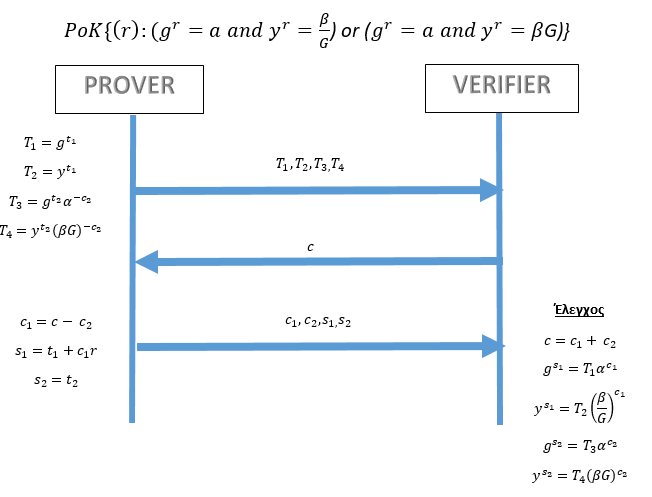
\includegraphics[scale=0.5]{cgs97.PNG}
    \end{center}
\end{frame}

\end{section} 

\begin{section}{Δίκτυα Μίξης}
\begin{frame}{Ψηφοφορίες με Δίκτυα Μίξης}{Εισαγωγή}
\begin{itemize}
    \item Γενικό δομικό στοιχεία για εφαρμογές ανωνυμίας \pause 
    \item Προτάθηκε από τον David Chaum (1981) \pause 
    \item Αποτελείται από ένα σύνολο από \textbf{μίκτες}. Κάθε ένας:
    \begin{itemize} \pause 
        \item λαμβάνει ένα σύνολο από μηνύματα (ΒΒ)
        \item αλλάζει τη μορφή τους
        \item εφαρμόζει μια τυχαία μετάθεση (ανακάτεμα)
    \end{itemize}
    \item Δύο μορφές λειτουργίας \pause 
    \begin{itemize}
        \item Σειριακά (κάθε μίκτης σε όλα τα μηνύματα)
        \item Παράλληλα (κάθε μίκτης σε ένα υποσύνολο από τα μηνύματα)
    \end{itemize} \pause 
    \item Στις ψηφοφορίες: τα μηνύματα είναι οι ψήφοι (ανακάτεμα της κάλπης)
    \item BB: παρέχει είσοδο και λαμβάνει έξοδο από κάθε μίκτη
\end{itemize}
\end{frame}

\begin{frame}{Γενική Μορφή Δίκτυου Μίξης}
    \begin{center}
        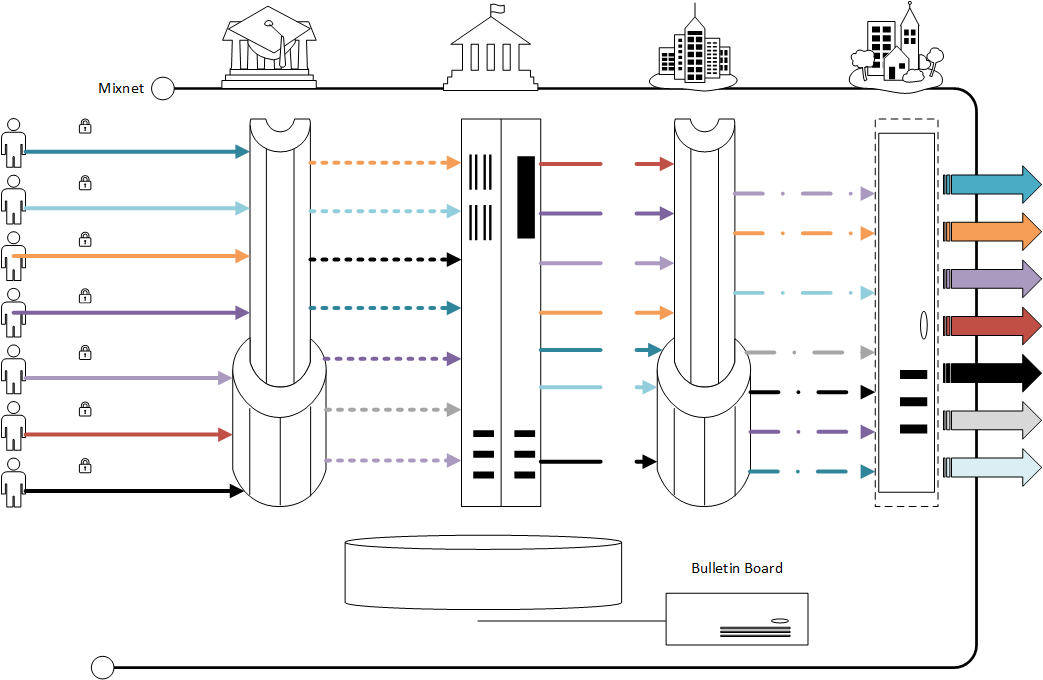
\includegraphics[scale=0.35]{mix.PNG}
    \end{center}
\end{frame}

\begin{frame}{Decryption Mixnets (RSA)}
\begin{itemize}
    \item Κάθε μίκτης $i$ έχει ένα ζεύγος κλειδιών RSA $(pk_i, sk_i)$ \pause 
    \item Ψηφοφόρος: κρυπτογράφηση ψήφου με δημόσια κλειδιά των μικτών \textit{σε αντίστροφη σειρά}. 
        \begin{center}
        $L_0 = \{ Enc_{pk_1}(Enc_{pk_2}( \cdots Enc_{pk_m}(v_i,r_i) \cdots, r_2), r_1) \}_{i=1}^n$
        \end{center}
    \item Μίκτης: Αλλαγή Μορφής \pause 
    \begin{itemize}
    \item αφαιρεί ένα επίπεδο κρυπτογράφησης χρησιμοποιώντας με το ιδιωτικό του κλειδί (ξεφλούδισμα)
    \item αφαιρεί την τυχαιότητα που περιέχει
    \item αλλάζει την μορφή.
    \end{itemize} \pause 
    \item Μίκτης: Ανακάτεμα \\ 
    \begin{itemize}
        \item Επιλογή τυχαίας μετάθεσης και εφαρμογή στα μηνύματα
        \item Το αποτέλεσμα γράφεται στο ΒΒ
        \item Για παράδειγμα ο πρώτος μίκτης θα γράψει:        
        \begin{center}
         $\ L_1 = \{ Enc_{pk_2}( \cdots Enc_{pk_k}(v_{i},r_{i}) \cdots, r_2) \}_{i=\pi_1(1)}^{\pi_1(n)} $
        \end{center}        
    \end{itemize} 
 \end{itemize}
 \end{frame}
 \begin{frame}{Decryption Mixnets (RSA)}
 \begin{itemize}
    \item Η διαδικασία επαναλαμβάνεται. \pause 
    \item Τελικά στην έξοδο  του δικτύου μίξης:
        \begin{center}
        $\ L_k = \{  v_{i} \}_{i=\pi_k \circ \cdots \circ \pi_1(1)}^{\pi_m \circ \cdots \circ \pi_1(n)}) $
        \end{center} \pause 
    \item Ακολουθεί η καταμέτρηση 
    \item Παρατηρήσεις: \pause 
        \begin{itemize}
            \item Αρκεί ένας `τίμιος' μίκτης απέναντι σε παθητικό αντίπαλο
            \item Ο τελευταίος μίκτης έχει πρόσβαση στο plaintext
            \item Το πλήθος των κρυπτογραφήσεων και το μέγεθος του κρυπτοκειμένου είναι ανάλογο του αριθμού των μικτών.
        \end{itemize}
\end{itemize} 
\end{frame}

\begin{frame}{Reencryption Mixnets (ElGamal)}
   \textbf{ Αλλαγή μορφής μηνυμάτων:} Reencryption
   \begin{center}
    $Enc(v, r_1) * Enc(0, r_2) = Enc(v,r_1+r_2)$
   \end{center} \pause 
    Δύο επιλογές:
    \begin{itemize}
        \item Μόνο Reencryption 
         Ο μίκτης $M_j$:
        \begin{itemize}
            \item Λαμβάνει από το ΒΒ την είσοδο \begin{center} $L_{j-1} = \{ (g^{r_{j-1,i}}, v_i \cdot y^{r_{j-1,i}}) \}_{i=1}^n$  \end{center} \pause
            \item Εισάγει νέα τυχαιότητα με reencryption:
            \begin{center}$L_{j-1} =  
    	        \{ (g^{r_{j-1,i}+r{j,i}}, v_i \cdot y^{r_{j-1,i}+r{j,i}}) \}_{i=1}^n $  
            \end{center} \pause
            \item Εφαρμόζει μία τυχαία μετάθεση $\pi_j$ \pause
            \item Γράφει τα αποτελέσματα στο BB
        \end{itemize} 
   \end{itemize} 
 \end{frame}
 
 \begin{frame}{Reencryption Mixnets (ElGamal)}
   \begin{itemize}  
        
        \item Αποκρυπτογράφηση και Reencryption\\
        $y_j$ είναι το δημόσιο κλειδί κάθε μίκτη  $M_j$ \\
        Κρυπτογράφηση με συνδυασμένο δημόσιο κλειδί  $\prod_{j=1}^k y_j$ \pause
        
        \begin{itemize} 
        \item Η είσοδος είναι:
        \begin{center}$L_0 = \{ (g^{r_{0i}}, v_i (y_1 \cdots y_k)^{r_{0i}}) \}_{i=1}^n$ \end{center} \pause

        \item Ο $M_j$ αποκρυπτογραφεί μερικώς 
        \begin{center}
        $L_{j-1} = \{ (g^{\sum_{t=0}^{j-1} r_{ti}}, v_i \cdot (\prod_{t=j}^k y_t)^{\sum_{t=0}^{j-1} r_{ti}}) \}_{i=1}^n$ 
        \end{center}
        διαιρώντας με $g^{x_j \cdot {\sum_{t=0}^{j-1} r_t}}$ \pause και εφαρμόζει νέα τυχαιότητα $r_{ji}$: 
        \begin{center}
        $L_{j} = \{ (g^{\sum_{t=0}^{j} r_{ti}}, v_i \cdot (\prod_{t=j+1}^k y_t)^{\sum_{t=0}^{j} r_{ti}}) \}_{i=1}^n$
        \end{center} \pause
        \item Εφαρμόζει μία τυχαία μετάθεση $\pi_j$ 
        \end{itemize} 
    \end{itemize} 
\end{frame}

\begin{frame}{Ενεργή επίθεση (Pfitzmann)}
    \begin{itemize}
\item Στόχος \adv: αποκάλυψη $v_i$ για συμμετέχοντα $P_i$ \pause  
\item Μέσο: Συνεργασία με κάποιο 'κακό' ψηφοφόρο \pause 
\item Ανάκτηση αρχικής ψήφου από το ΒΒ  \pause 
\begin{center}
$c_{i0} = (g^R, v_i \cdot (y_1,\cdots,y_k)^R) = (t,u)$ 
\end{center}
\item Ο  \adv επιλέγει τυχαίο $x$ και παράγει \pause 
\begin{center}
$c^{''}_{i0} = (t^x,u^x)=( g^{R'x}, v_{i}^{x} \cdot (y_j,\cdots,y_k)^{R'x} )$ 
\end{center}
\item Αντικατάσταση ψήφου του συνεργάτη του. \pause 
\item Η έξοδος του δικτύου μίξης θα περιέχει  το $v_{i}^{x}$  και $v_{i}$ \pause 
\item Ο \adv ανακτά όλα τα μηνύματα εξόδου και τα υψώνει στην $x$. \pause 
\item Στην συνέχεια ελέγχει τις δύο λίστες για κοινά στοιχεία. \pause 
\item Όταν βρει έμαθε το μήνυμα που έψαχνε καθώς $v_{\pi(i)}^x = v_i^x$. 
\end{itemize}
\end{frame}

\begin{frame}{Λύσεις}
Επαληθευσιμότητα των ενεργειών ψηφοφόρων και μικτών \pause 
\begin{itemize}
  \item Ψηφοφόρος: Απόδειξη γνώσης της ψήφου ώστε 
  \begin{itemize}
   \item να \textbf{μην} βάλει ετικέτα σε κάποια ψήφο
   \item να \textbf{μην}  αντιγράψει μια ψήφο
  \end{itemize} \pause 
  \item Όπως στα ομομορφικά συστήματα \pause 
  \item Μίκτης: Απόδειξη μετάθεσης (proof of shuffle)
  \begin{itemize}
   \item Η μετάθεση είναι έγκυρη
   \item χωρίς να αλλάξει κάποια ψήφο
   \item χωρίς να παραλείψει κάποια ψήφο 
  \end{itemize}
\end{itemize}
\end{frame}
 
\begin{frame}[allowframebreaks]{Παράδειγμα}{Προσθήκη επαληθευσιμότητας σε ένα απλό δίκτυο μίξης} 

\begin{multicols}{2}
    \begin{itemize}
        \item Έισοδος: 
        \begin{itemize}
            \item  $C_1 = Enc(m_1,r_1)$
            \item $C_2 = Enc(m_2,r_2)$.
        \end{itemize}
        
        \item Reencryption
          \begin{itemize}
        \item ${C'}_1 = Reenc(C_1)=Enc(m_1,r_1+r_1')$ \item ${C'}_2 = Reenc(C_2)=Enc(m_2,r_2+r_2')$
           \end{itemize}
        \item Tυχαία επιλογή bit $b \in_R \{0,1\}$.
        \item Αν $b=0$ έξοδος $({C'}_1, {C'}_2)$ 
        \item Αν $b=1$ έξοδος $({C'}_2, {C'}_1)$
    \end{itemize}
    \vfill \columnbreak
    \begin{figure}
        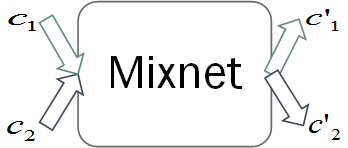
\includegraphics[scale=0.5]{mix2x2.PNG}
    \end{figure}
\end{multicols}

\framebreak
 
\textbf{Βήμα 1} Απόδειξη ορθότητας reencryption 

\begin{block}{Δηλαδή}
Το κρυπτογράφημα ${C'} = (G',M') = (g^u,m' \cdot y^u)$ είναι reencryption του $C = (G,M) = (g^t,m \cdot y^t)$
\end{block}

\textbf{Βασική ιδέα:} Το ${C'}$ είναι reencryption του $C$ ανν και τα δύο κρυπτογραφούν το ίδιο μήνυμα, δηλ. $m'=m$.

Διαιρούμε τα δύο μέρη και έχουμε:
\begin{center}
$\frac{G'}{G}=\frac{g^u}{g^t}=g^{u-t}$ και 
$\frac{M'}{M}=\frac{m' y^u}{m y^t}=y^{u-t}$ 
\end{center}

Αρκεί νδο ότι $ log_g \frac{G'}{G} = log_y \frac{M'}{M}$

Χρήση non interactive Chaum Pedersen

\framebreak

\begin{block}{\textbf{Βήμα 2} Απόδειξη ορθότητας μετάθεσης }
Πρέπει νδο $\{C'_1,C'_2\}$ είναι reencryption μια μετάθεσης του $\{C_1,C_2\}$ χωρίς να την φανερώσουμε την αντιστοιχία. \\
\end{block}
 

Ισοδύναμα:
\begin{center}
$(C'_1 = Reenc(C_1) \wedge C'_2 = Reenc(C_2)) \bigvee (C'_1 = Reenc(C_2) \wedge C'_2 = Reenc(C_1))$
\end{center}

 
\textbf{Λύση}: Σύνθεση 4 πρωτοκόλλων Chaum-Pedersen
 
\end{frame}
\end{section} 

\begin{section}{Ψηφοφορίες με Τυφλές Υπογραφές}


\begin{frame}{Ψηφοφορίες με Τυφλές Υπογραφές}{Γενική μορφή}
\begin{itemize}
\item Ο ψηφοφόρος υποβάλλει μία `τυφλωμένη' έκδοση του ψηφοδελτίου μαζί με πληροφορίες ταυτότητας.  \pause 
\item Η εκλογική αρχή επαληθεύει την ταυτότητα του υποψηφίου και ελέγχει αν έχει δικαίωμα ψήφου. Αν η απάντηση είναι θετική υπογράφει ψηφιακά το τυφλωμένο ψηφοδέλτιο και το επιστρέφει στον ψηφοφόρο. \pause 
\item Ο ψηφοφόρος αφού επαληθεύσει την υπογραφή της αρχής καταθέτει το ψηφοδέλτιο στο BB \textit{ανώνυμα}.  \pause 
\item Η αρχή λαμβάνει τα υπογεγραμμένα ψηφοδέλτια και επαληθεύει την υπογραφή της. \pause 
\item O ψηφοφόρος μπορεί να επαληθεύσει το ψηφοδέλτιο του εισάγοντας σε αυτό ένα τυχαίο αριθμό που μόνο αυτός γνωρίζει. 
\end{itemize}

\end{frame}


\begin{frame}{Fujioka, Okamoto και Ohta (FOO92)}
    \begin{center}
        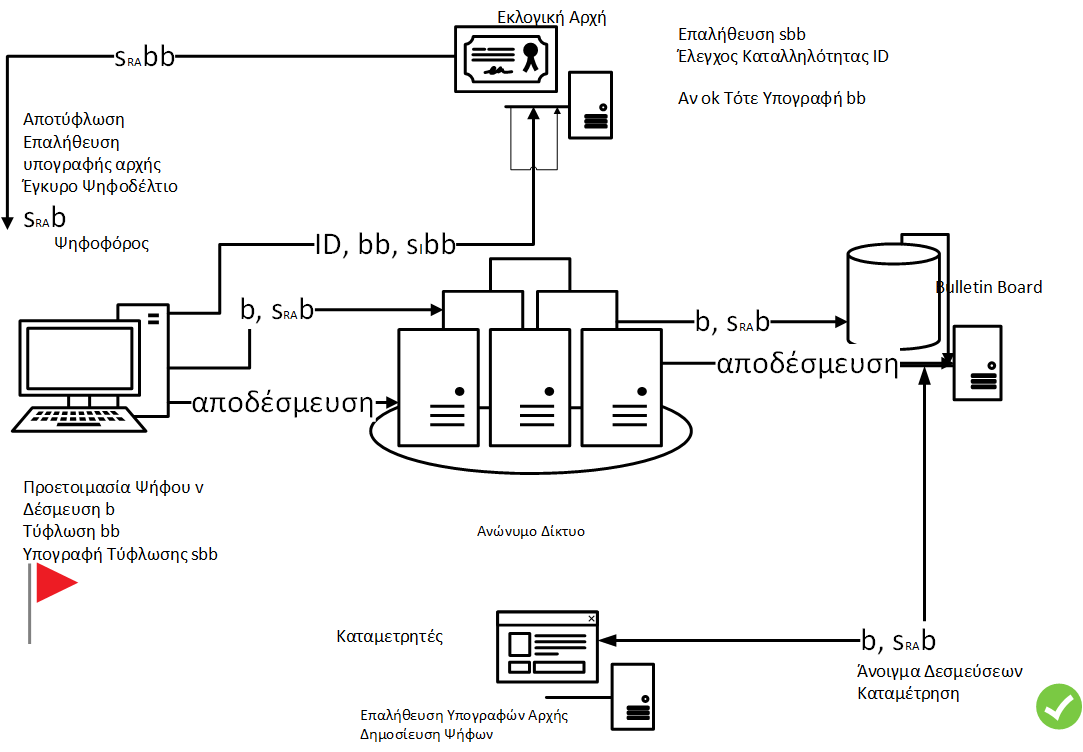
\includegraphics[scale=0.35]{foo.PNG}
    \end{center}
\end{frame}

\begin{frame}[allowframebreaks]{Αναλυτική περιγραφή}

\begin{enumerate}
\item \textbf{Ψηφοφόρος: Προετοιμασία}
\begin{itemize}
\item Επιλογή ψήφου $v_i$
\item Δέσμευση στην ψήφο με τυχαιότητα $rc_i$. Το ψηφοδέλτιο είναι: $b_i = commit(v_i, rc_i) = g^{rc_i} h^{v_i}$. 
\item Τύφλωση του ψηφοδελτίου με $rb_i$ και δημόσιο κλειδί της αρχής  $bb_i = blind(b_i,rb_i) = b_i rb_{i}^{e_A}$.
\item Υπογραφή $sbb^I_i = sign_{d_I}(bb_i)$.
\item Αποστολή $(id_i,bb_i,sbb^I_i)$ στην εκλογική αρχή (RA)
\end{itemize}

\framebreak

\item \textbf{RA:Εξουσιοδότηση}
\begin{itemize}
\item Έλεγχοι: 
\begin{itemize}
    \item υπογραφή του ψηφοφόρου
    \item το δικαίωμα του να ψηφίσει 
    \item αν έχει διπλοψηφίσει
\end{itemize}  
\item Επιτυχείς έλεγχοι $\rightarrow$ έγκριση μέσω υπογραφής του τυφλωμένου ψηφοδελτίου $sbb_i^A = sign_{d_A}(bb_i) = b_i^{d_A} rb_{i}$.
\item Τέλος επιστρέφει το $sbb_i^A$ στον ψηφοφόρο $i$
\item Ανακοίνωση από RA του συνολικού αριθμού ψηφοφόρων.
\end{itemize}

\framebreak

\item \textbf{Ψηφοφορία: Ενέργειες Ψηφοφόρου}
\begin{itemize}
\item Αποτύφλωση υπογεγραμμένου ψηφοδελτίου $sb_i^A = unblind(sbb^i_A)=b_i^{d_A}$
\item Επαλήθευση υπογραφής από όλους
\item Κατάθεση ψήφου: Αποστολή των $b_i,sb_i^A$ στην αρχή καταμέτρησης
\item Χρήση ανώνυμου καναλιού (πχ. δίκτυο μίξης) για απόκρυψη στοιχείων που ίσως προδώσουν την ταυτότητα του ψηφοφόρου (πχ. δικτυακές διευθύνσεις).
\end{itemize}

\framebreak

\item \textbf{Καταμετρητές: Συλλογή}
\begin{itemize}
\item Η αρχή καταμέτρησης επαληθεύει την υπογραφή της αρχής σε κάθε ψηφοδέλτιο $sb_i^A$.
\item Όσα ψηφοδέλτια πέρασαν τον έλεγχο δημοσιεύονται σε μια λίστα $\{ idx, b_i, sb_i^A \}$.
\end{itemize}

\framebreak

\item \textbf{Αποδεσμεύσεις - Επαληθεύσεις}
Λήξη προθεσμίας ψηφοφορίας κάθε ψηφοφόρος (και λοιποί ενδιαφερόμενοι) επαληθεύουν:

\begin{itemize}
\item το ψηφοδέλτιο καθενός βρίσκεται στο BB.
\item το πλήθος των ψηφοφόρων που δημοσίευσε η εκλογική αρχή =   πλήθος των ψηφοδελτίων που δημοσίευσε η αρχή καταμέτρησης. 
\item Επιτυχείς έλεγχοι $\Rightarrow$ αποστολή $idx,rc_i$ μέσω ανώνυμου καναλιού
\item Άνοιγμα δεσμεύσεων από καταμετρητές
\end{itemize}
  
\item \textbf{Καταμέτρηση}
\begin{itemize}
\item Δημοσίευση 'ανώνυμων' ψηφοδελτίων
\item Καταμέτρηση από κάθε ενδιαφερόμενο  
\end{itemize}
\end{enumerate}

\end{frame}
\end{section} 
 
\begin{frame}{Ανοιχτά Θέματα} 
\begin{adjustwidth}{-2em}{-2em}
    \begin{multicols}{2}
    \begin{small}
    \begin{itemize}
    \setlength\itemsep{0.1em}
        \item Θέματα υλοποίησης
        \begin{itemize}\setlength\itemsep{0.1em}
            \item Κωδικοποίηση πολλών υποψηφίων
            \item Απόδοση NIZKP (μέγεθος, ταχύτητα δημιουργίας και επαλήθευσης)
        \end{itemize} \pause
        \item Everlasting privacy
        \begin{itemize}\setlength\itemsep{0.1em}
            \item Adi Shamir: Όλα τα κρυπτογραφικά κλειδιά που χρησιμοποιούνται σήμερα θα είναι άχρηστα σε 30 χρόνια
            \item Quantum Computing
            \item Λόγω verifiability οι ψήφοι είναι εν δυνάμει διαθέσιμοι σε πολλές οντότητες
        \end{itemize} \pause
        \columnbreak
        \item Εναλλακτικές μέθοδοι υπολογισμού αποτελέσματος
        \begin{itemize}\setlength\itemsep{0.1em}
            \item σε συνδυασμό με ομομορφικά συστήματα
        \end{itemize} \pause
        \item Coercion resistance 
        \begin{itemize}\setlength\itemsep{0.1em}
            \item Απαραίτητο για internet voting
            \item Κάθε ψηφοφόρος: Δυνατότητα πολλών επιλογών
            \item Εκβιαστής: Δεν μπορεί να αποφανθεί αν πέτυχε η προσπάθειά του
        \end{itemize}
    \end{itemize}
    \end{small}
    \end{multicols}
    \end{adjustwidth}
\end{frame}

\begin{frame}[allowframebreaks]{Βιβλιογραφία}
\begin{tiny}
\begin{itemize}
 \item B. Adida. Advances in cryptographic voting systems. PhD thesis, Massachusetts Institute of Technology, 2006.
 \item David Chaum. Untraceable electronic mail, return addresses, and digital pseudonyms. Commun. ACM, 24(2):84--88, 1981.
 \item David Chaum. Blind signatures for untraceable payments. In D. Chaum, R.L. Rivest, and A.TSherman, editors, Advances in Cryptology Proceedings of Crypto 82, pages 199--203, 1983.
 \item Josh D. Cohen and Michael J. Fischer. A robust and verifiable cryptographically secure election scheme (extended abstract). In FOCS, pages 372--382, 1985.
 \item Ronald Cramer, Rosario Gennaro, and Berry Schoenmakers. A secure and optimally efficient multi-authority election scheme. pages 103--118. Springer-Verlag, 1997
 \item J. Alex Halderman. Securing digital democracy. Coursera Online Course, September 2012.
 \item Ari Juels, Dario Catalano, and Markus Jakobsson. Coercion-resistant electronic elections. In Proceedings of the 2005 ACM workshop on Privacy in the electronic society, pages 61--70.
ACM, 2005. 
 \item Atsushi Fujioka, Tatsuaki Okamoto, and Kazuo Ohta. A practical secret voting scheme for large
scale elections. In Proceedings of the Workshop on the Theory and Application of Cryptographic
Techniques: Advances in Cryptology, ASIACRYPT '92, pages 244--251, London, UK, UK,
1993. Springer-Verlag.
 \item ABE Masayuki. Mix-networks on permutation networks. In ASIACRYPT’99, page 258. Springer.
 \item Choonsik Park, Kazutomo Itoh, and Kaoru Kurosawa. Efficient anonymous channel and all/nothing election scheme. In EUROCRYPT, pages 248--259, 1993.
  \item B. Pfitzmann and A. Pfitzmann. How to break the direct rsa-implementation of mixes. In Advances in Cryptology—EUROCRYPT’89, pages 373--381. Springer, 1990
\end{itemize} 
\end{tiny}
\end{frame}

\end{document}